\section{The adaptive prolongation approach}

\subsection{HARP}
\todo{Explanation of the general structure of HARP, without going into detail about the coarsening procedure}
HARP is a method for improving the performance of graph representation learning (i. e. graph embedding) algorithms such as DeepWalk \cite{perozzi_deepwalk_2014}, LINE \cite{tang_line_2015}, PTE \cite{tang_pte_2015} or node2vec \cite{grover_node2vec_2016}. The method is a combination of dataset augmentation and pre-training based on the general principle that graph-based models train more efficiently on smaller graphs and can thus be pre-trained on a coarsened representation of the graph at hand. Moreover, the coarsened graphs approximate the global structure of the original data, enabling the representations to better encapsulate such a global structure. In an overview, the method consists of the following steps:

\begin{itemize}
  \item \textbf{Dataset augmentation}. The graph is consecutively reduced in size by the application of several graph coarsening schemas. In each step, the coarsened graph can be viewed as an ever coarser representation of the graph data and its global structure.
\end{itemize}
After all the coarsened graphs are pre-computed, the method itself can be executed by repeating the following steps on the graphs from the coarsest to the finest:
\begin{itemize}
  \item \textbf{Training on an intermediary graph}. The model is trained on one of the pre-computed intermediary graphs.
  \item \textbf{Embedding prolongation}. The embedding generated by the model is prolonged from a coarser graph to a finer one (with the original graph being the finest).
\end{itemize}

The first step is independent of the rest of the computation and can be done ahead of time. The last two steps can be seen as a form of pre-training for the model that is to be learnt on the original graph. The whole HARP pipeline is demonstrated in Figure \ref{fig:harp-overview}.

\begin{figure}
  \centering
  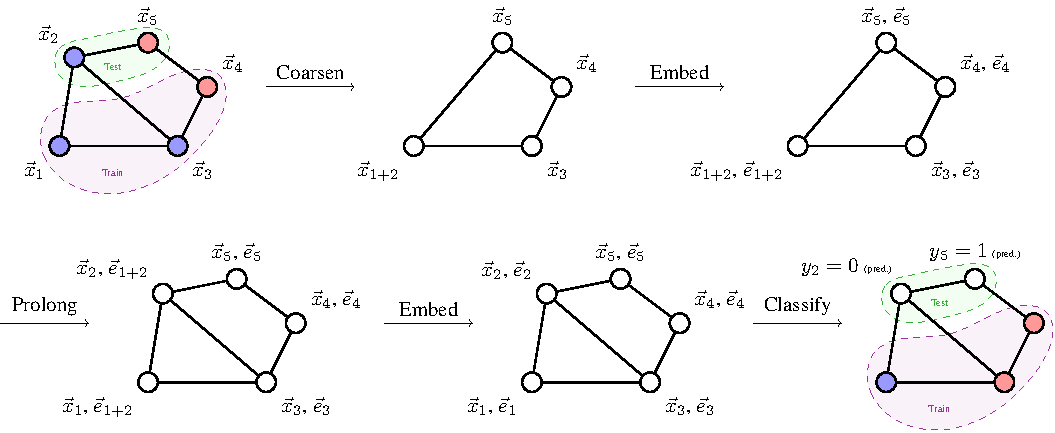
\includegraphics[width=\linewidth]{images/harp-overview/harp-overview.pdf}
  \caption{An overview of the HARP processing pipeline with one level of coarsening}
  \label{fig:harp-overview}
\end{figure}

\subsection{Balancing performance and complexity}

\todo{This is WIP and needs to be rewritten after next subsection is done}
Graph-based methods such as node2vec typically have a large number of parameters - on the widely used OGBN-ArXiv\todo{Don't mention OGB if no evaluation on OGB} dataset (see \cite{hu_open_2021}), the state-of-the-art node2vec model has over 21 million parameters. At the same time, recent works in the domain of graph learning have started to focus more heavily on simpler methods as a competitive alternative to heavy-weight ones (see \cite{frasca_sign_2020,huang_combining_2020,salha_keep_2019,zhang_eigen-gnn_2020}). As the authors of \cite{chen_harp_2018} observed, HARP improves the performance of models when fewer labelled data are available. The proposed lower complexity models based on HARP could also improve performance in a setting where only low fidelity data are available for large parts of the graph. Coarser models could be trained on them, with a subsequent training of finer models using only a limited sample of high fidelity data.

\subsection{Our method}
Explanation of the adaptive prolongation approach
